%2345678901234567890123456789012345678901234567890123456789012345678901
\chapter{Data Provenance} % (fold)
\label{cha:data_provenance_in_the_vo}

	%\section{Introduction} % (fold)
	%\label{sec:vo_provenance_introduction}
	%
	%% section vo_provenance_introduction (end)

	\attributedquote{
		\dictionarydef
			{provenance}
			{noun}
			{
				\begin{itemize}
					\item the place of origin or earliest known
					history of something.
					
					\item the beginning of something's existence;
					something's origin.
					
					\item a record of ownership of a work of art
					or an antique, used as a guide to authenticity
					or quality.
				\end{itemize}
			}
	}
	{The New  Oxford American Dictionary, \emph{2nd Edition}}
	
	\noindent
	The dictionary definition above points to the main three
	elements to which data provenance in e-Science has to deal
	with: Attribution, i.e. proper acknowledgement of authorship
	and or origin; Data Quality; and Replication of results, i.e.,
	the chain of processes needed to derive a result, beginning
	with data sources.
	
	 In the VO context, we can synthesise a definition by stating
	that Provenance (data provenance) is the record of the earliest
	known history of an astronomical data set, to be used as a
	guide to data quality and of data ownership.
	
	 Astronomical datasets use the data coming from different
	photons\footnote{Their arrival rate, their energy distribution,
	the positions from the sky, the difference with properties of
	photons not coming from the observed region; in addition, the
	response to photons, and to their absence, has also to be
	determined.} to derive physical properties from the observed
	objects. Therefore, data provenance ---also known as
	\emph{lineage} information--- in astrophysics is, in fact, the
	answer to the question \emph{What was done to this collection
	of photons, and which systems did it?}
	
	\section{Provenance in e-Science} % (fold)
	\label{sec:provenance_in_escience}
	
		As we have already established, data Provenance in the
		Virtual Observatory is just a specific form of the
		problem of data Provenance in e-Science, so in order
		to establish how to model astronomical data provenance,
		we will study first the different data provenance
		recording and determination techniques already
		available.
		
		\begin{figure}[tbp]
			\centering
				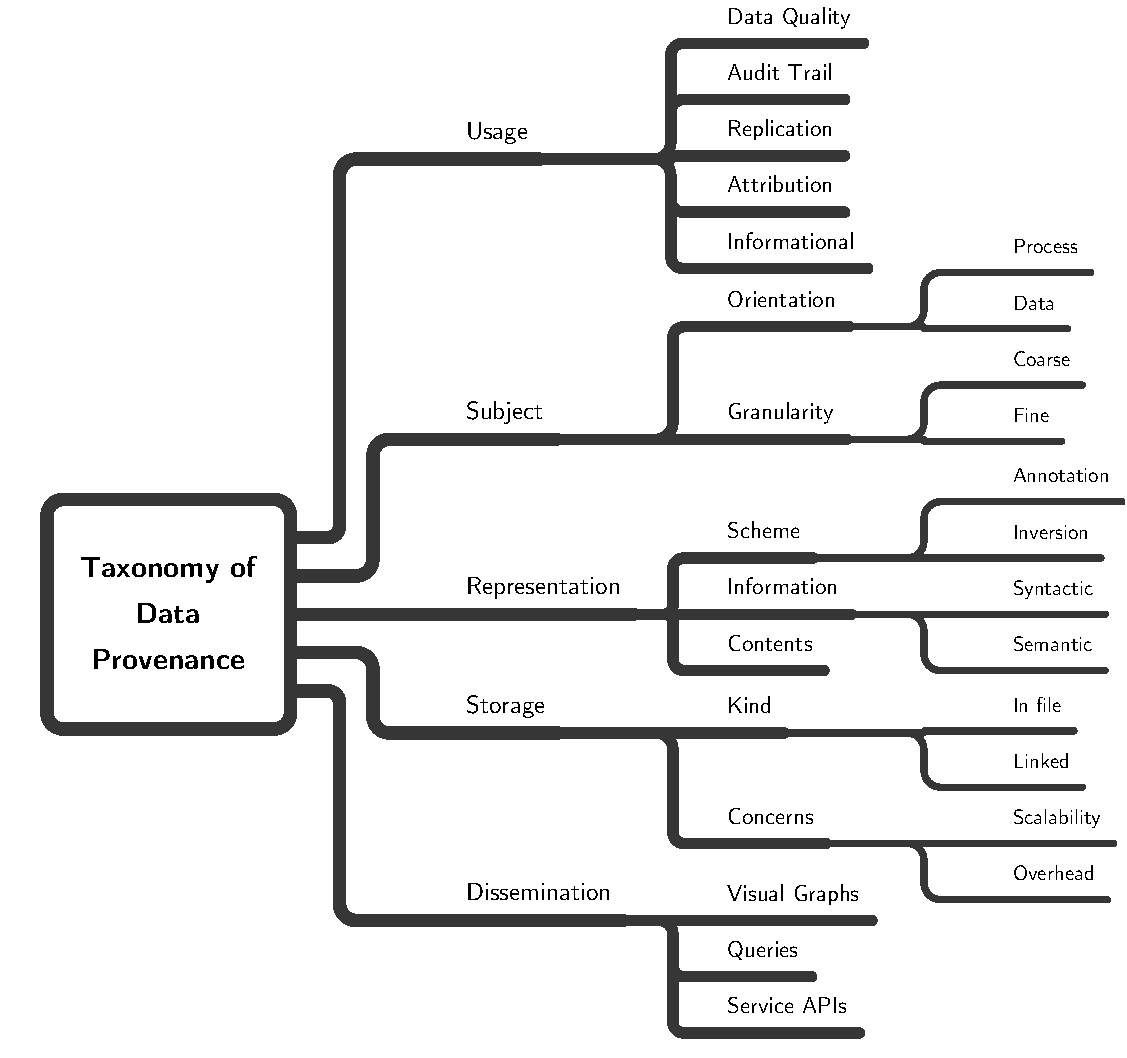
\includegraphics[width=\columnwidth]
				{fig/DataProvenanceTaxonomy.pdf}
			\caption[
				Taxonomy of data provenance techniques in
				e-Science
			]
			{
				Taxonomy of data provenance techniques in
				e-Science. Those techniques can be classified
				depending on the use of the provenance data
				collected, on the actual subject of data
				provenance, or the way data provenance is
				represented, stored, or disseminated. Based on
				\emph{A Survey of Data Provenance in
				e-Science}~\cite{SimPlaGan0503A-Survey}.
			}
			\label{fig:fig_DataProvenanceTaxonomy}
		\end{figure}
		
		In the paper \emph{A Survey of Data Provenance in
		e-Science}~\cite{SimPlaGan0503A-Survey} by Simmhan et al.
		many different data provenance collection techniques are
		studied, and a taxonomy of them is created ---see
		figure~\ref{fig:fig_DataProvenanceTaxonomy}---, depending
		on:
		
		\begin{description}
			\item[Usage] Data provenance information can be used
			for estimating data quality and data reliability, or to
			provide an audit trail of the data transformations. It
			can also be used to replicate an experiment, to
			attribute the creation of a dataset to a set of
			original (in the sense of originating) data, and to the
			set of processes needed to derive the new dataset. Or
			it can be informational, without providing enough
			information to assess any of the above.
			
			\item[Subject] Data provenance can be focused on the
			data themselves, collecting lineage metadata from each
			data product, or on the processes on the data. And in
			any case the recorded provenance can be coarse grained
			(for instance, describing a whole set of data) or fine
			grained (describing each single datum and/or process;
			for instance, database tuples' attributes).
			
			\item[Representation] The way data provenance can be
			represented is also diverse, and some of them depend on
			the processing system being studied. The two main
			approaches in the literature are annotations and
			inversion. Annotations are \emph{a priori} provenance
			metadata: the transformed data are accompanied by
			provenance metadata which has been created prior to the
			transformation. On the other hand, inversion data
			provenance is created \emph{a posteriori} from the data
			products of a transformation which can be inverted,
			with provenance metadata being created from the
			documentation of the process and the differences
			between inputs and outputs. It is clear that inversion
			metadata are more compact, while annotations can
			include parameters of processes, their versions, and
			even references to publications.
			
			 As some of the lineage information implies
			relationships between datasets and processes, that
			information can be captured in data models about the
			processes, or using semantic web technologies, such as
			the RDF and OWL languages, in order to describe such
			relationships. In this way, the process semantics are
			documented. In any case, the process syntax is
			specified from the input data, the output data, and
			annotations, if present.
			
			\item[Storage] As provenance metadata can be generated,
			collected and/or transmitted at many different places,
			there must be a way to keep those metadata stored,
			while keeping the relationship with the data
			themselves. Depending on the grain of the metadata
			collection process, and on whether the lineage
			information is just updated or versioned, the amount of
			provenance metadata can grow several orders of
			magnitude above the original data. Both the overhead of
			provenance metadata (percentage of storage devoted to
			provenance versus data, and cost of metadata
			management), and the scalability of the system, that
			is, how to deal with the provenance metadata if the
			data rate increases an order of magnitude.
			
			\item[Dissemination] Finally, provenance metadata are
			gathered for applications to use them. Typical ways of
			disseminating lineage information are by means of
			derivation graphs~\todoinlinesuspended{\citeneeded},
			but in many cases where
			the provenance metadata are stored inline with the data
			the form is just a list of time-stamped annotations. If
			semantic web tools are used, workflows can determine
			the input provenance information and create the
			dissemination graph at runtime. In addition, specially
			in cases were lineage metadata are stored in databases
			or XML documents, provenance specific queries can be
			performed, and even provenance query APIs can be created
			so that different systems can access such information.
			
		\end{description}
	
		Another classification~\cite{Buneman:2001fc}
		of Provenance data can be performed regarding how it
		is collected or computed:
		
		\begin{description}
			\item[Why provenance] Refers to the reason why a datum
			is in a given dataset, i.e., the query that was
			performed, including data sources. For data coming from
			database queries, different fields can have different
			sources, but all fields, and many rows derived from the
			same query, will share that query. In a sense,
			\emph{Why} provenance is a proof that a datum belongs
			to a processed (queried) data set, as it corresponds to
			the minimum set of sources and sources' entries which,
			together with the query being performed, will provide
			that datum as an answer.
			
			\item[Where provenance] Refers to the actual
			progenitors of each particular datum, i.e., what
			particular database tuple, and field in the tuple,
			provided the datum we are analysing.
		\end{description}
		
		The difference between both kinds can be better illustrated
		using a database originated example.
		Let us imagine the SQL query:
		
		\begin{adjustwidth}{\parindent}{\parindent}
			\noindent\texttt{SELECT name, telephone\\
			FROM employee\\
			WHERE salary > (SELECT AVERAGE salary FROM employee)}
		\end{adjustwidth}
		
		 And let us say one of the tuples in the result is
		\texttt{("John Doe", 555123467)}. As all rows in
		\texttt{employee} where needed for the calculation of the
		salary average, a change in any row could make our target
		tuple disappear from the result list, so the \emph{Why}
		provenance is the query plus the \texttt{salary},
		\texttt{name} and \texttt{telephone} fields of all rows of
		the \texttt{employee} table. The \emph{Where} provenance,
		however, is only concerned with the actual progenitor of
		each of the tuple's datum, and the answer is the
		\texttt{name} and \texttt{employee} fields of the row
		containing John Doe's entry in the \texttt{employee} table.
		
		Finally, another difference can be established for
		data provenance collection systems, depending on the
		data collection strategy:
		
		\begin{description}
			\item[Eager collection] Lineage information is
			created/computed after each transformational or
			derivational step.
			
			\item[Lazy collection] Provenance information is
			calculated on demand, using specific knowledge of
			the transformations, and parameters saved.
		\end{description}
		
		We will end up our review
		of data provenance systems and classifications
		by showing table~\ref{provenanceSystems} of
		different data provenance management systems in different
		application areas, and see their characteristics.
		
		We can see that most
		of the systems assume a relational database
		infrastructure, and rely on annotations for carrying
		on provenance information. Only systems completely
		contained within a relational database systems use
		inverse queries or functions for their recovery of
		data provenance.
		
		\begin{sidewaystable}
		\begin{minipage}{\linewidth}
		\caption[Data provenance management systems' properties]
		{
			Properties of different data provenance management
			systems for different scientific domains, as compiled
			by~\cite{SimPlaGan0503A-Survey}.
		}
		\label{provenanceSystems}
		\begin{scriptsizetabular}
		{p{2.25cm} p{1.66cm} p{1.66cm} p{1.66cm} p{1.66cm} 
		 p{1.66cm} p{1.66cm} p{1.66cm} p{1.66cm} p{1.66cm}}
		
			& \textbf{LIP} & \textbf{Chimera} & \textbf{myGRID} &
			\textbf{CMCS} & \textbf{PASOA} & \textbf{ESSW} &
			\textbf{Tioga} & \textbf{Buneman} & \textbf{Trio} \\
			\midrule
			
			Domain\footnote{GIS: Geographical Information System}
			& GIS & Physics, Astronomy & Biology & Chemistry &
			Biology & Earth Sciences & Atmospheric Sciences &
			Generic & Generic \\ \addlinespace
			
			Processing\footnote{RDBMS: Relational Data Base
			Management System} & Commands & Services & Services &
			Services & Services & Scripts & RDBMS & RDBMS & RDBMS
			\\ \addlinespace
			
			Application\footnote{Kind of Provenance application:
			I: Informational; R: Regeneration; A: Audit; E: Error
			Tracking; U: Information Update; P: Planning} & IR &
			IRAP & IR & IU & IR & I & IE & IU & IU \\
			\addlinespace
			
			Orientation & Data & Process & Process & Data &
			Process & Data \& Process & Data & Data & Data \\
			\addlinespace
			
			Granularity & Spatial layers & Abstract datasets
			(files) & Abstract resources & Files & Workflow
			Parameters & Files & DB Attributes & DB Attributes \&
			Tuples & DB Tuples \\ \addlinespace
			
			Representation & Annotations & Annotations &
			Annotations & Annotations & Annotations & Annotations
			& Inverse functions & Inverse queries & Inverse
			queries \\ \addlinespace
			
			Semantics & No & No & Yes & Limited & No & Proposed &
			No & No & No \\ \addlinespace
			
			Storage\footnote{RDBMS: Relational Data Base
			Management System; N/A: Not available} & RDBMS & RDBMS
			& RDBMS & RDBMS & RDBMS + File System & RDBMS & RDBMS
			& N/A & RDBMS \\ \addlinespace
			
			Overhead & user commands; MD entry & user definition;
			automatic WF & service semantics; WF calls & service
			calls; working portal & manual & manual & manual
			registry of inverse functions & N/A & Automatic
			generation of inverse queries \\ \addlinespace
			
			Scalability & No & Yes & No & No & Proposed &
			Proposed & Yes & N/A & No \\ \addlinespace
			
			Dissemination\footnote{N/A: Not Available} & Queries
			& Queries & Semantic browser; Lineage graph & Queries;
			Browsing & Queries & Browsing & Queries; Graph & N/A &
			Queries
		\end{scriptsizetabular}
		\end{minipage}
		\end{sidewaystable}
		
		So, in order to establish a Data Provenance framework for
		the Virtual Observatory we will have to establish all of
		the items above: how to collect the information, which will
		be the intended use, and how is the information going to be
		represented, stored, and presented to intended users and
		systems; whether we need a \emph{Why} or \emph{Where}
		provenance system depending on typical VO use cases; and if
		such system must be \emph{Eager} or \emph{Lazy}, again
		depending on use cases.
		
	% section provenance_in_escience (end)

	\section{Provenance in astronomy and astrophysics} % (fold)
	\label{sec:provenance_in_astronomy_and_astrophysics}

		After the classification above, we will study the different
		data provenance techniques in use within the astronomy,
		together with their intended application.
		
		Typically, one of the uses of header cards in FITS files is
		storing \texttt{COMMENTS} and \texttt{HISTORY} cards.
		Figure~\ref{fig:fig_FITSHeadersProvenance} shows an example
		of a FITS file processed by the
		AIPS\urlnote{http://www.aips.nrao.edu/} interferometric
		data reduction software.
		
		\begin{figure}[tbp]
			\centering
				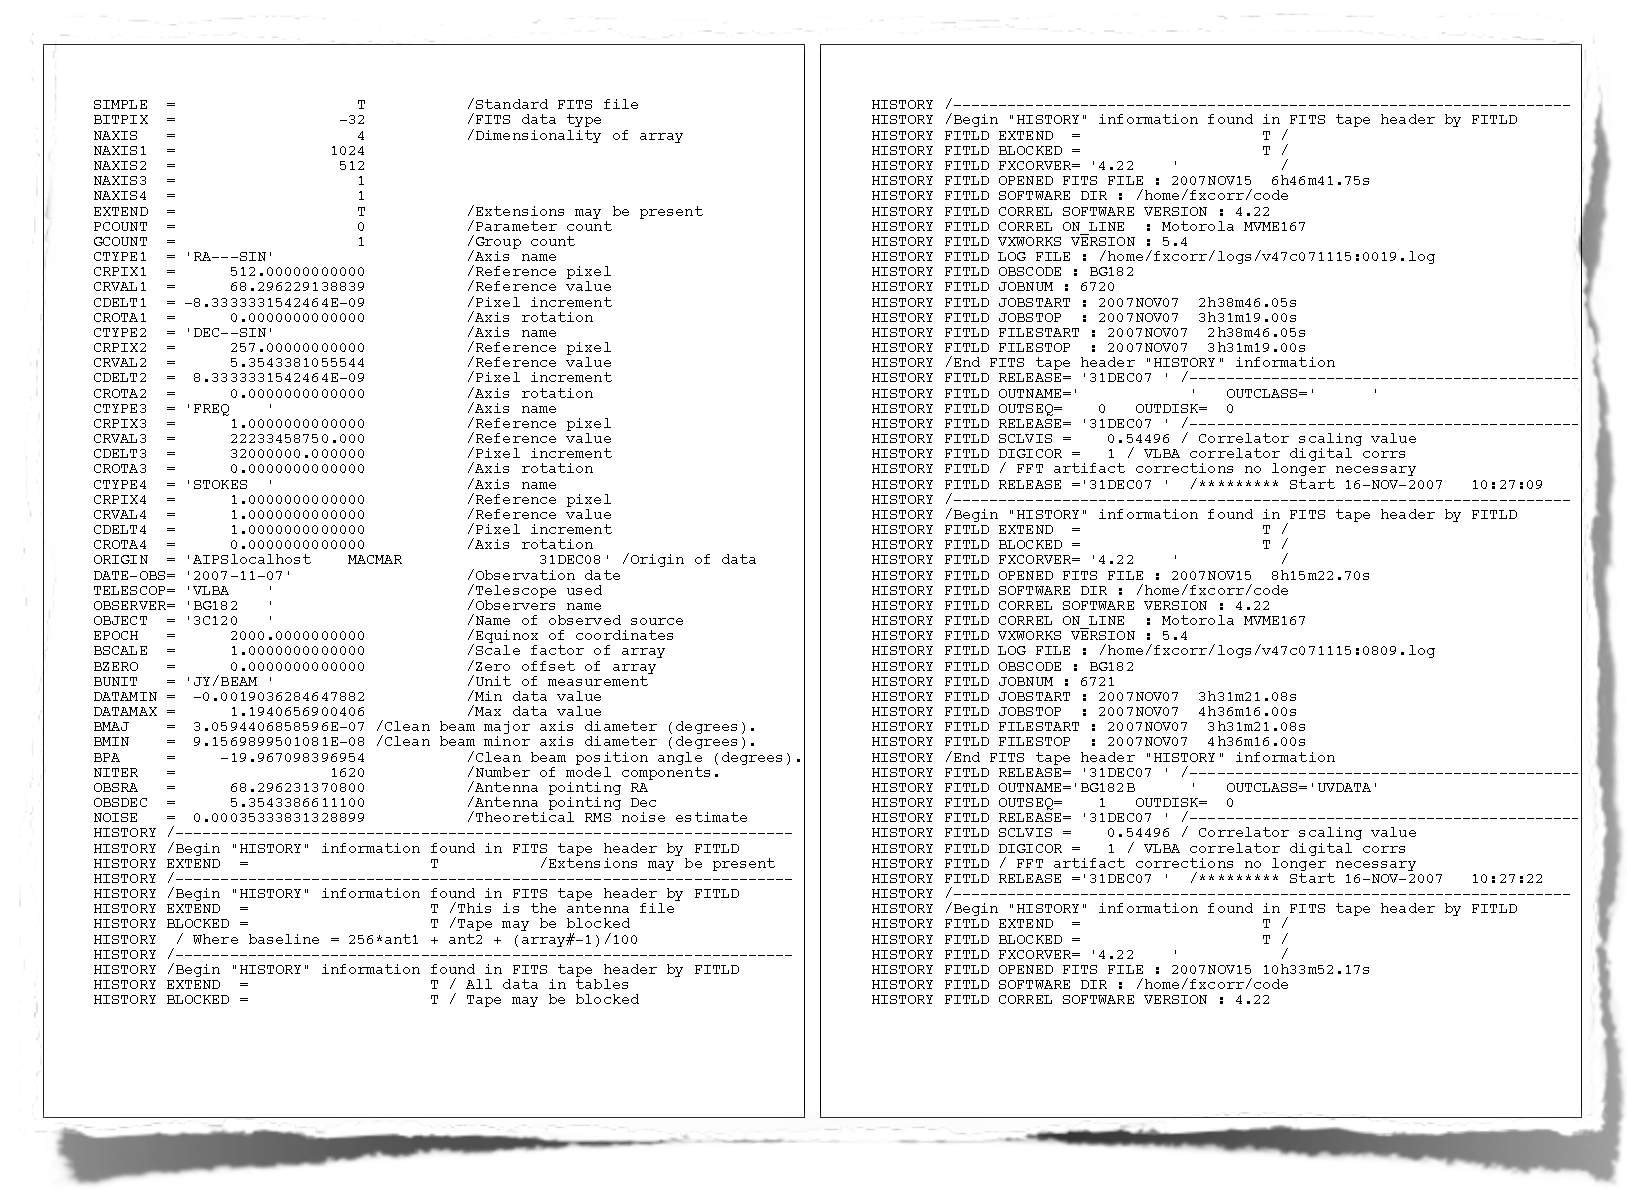
\includegraphics[width=\columnwidth]
				{fig/FITSHeadersProvenance.pdf}
			\caption[FITS headers showing AIPS History]{
				A pair of pages of FITS headers from a file which
				has been processed with the AIPS radio
				interferometry data reduction and imaging software.
				The first page starts with the headers establishing
				the axes for the observation (RA, Dec, Frequency
				and a fixed polarisation), and after that
				\texttt{HISTORY} tags start documenting the
				different calls to different AIPS tasks
				(\texttt{FITLD}, FITS LoaD, is the first one
				called by AIPS in order to create the AIPS data
				structures from the contents of the FITS file).
			}
			\label{fig:fig_FITSHeadersProvenance}
		\end{figure}
		
		In that figure we can see an example of how typical
		astrophysical tools have been dealing with data provenance.
		Each different application can make use of the FITS header
		cards, specifically of the \texttt{HISTORY} keyword, in
		order to provide feedback of the steps being performed on
		the data.
		
		 In this case, the data provenance being provided is of the
		\emph{Why} kind, albeit not complete. Apart from the text
		\emph{annotation} on the FITS headers, tables of task
		Parameters are stored within the FITS file itself, so this
		provenance information is collected \emph{eagerly}, and
		corresponds to \emph{Why} provenance. If all the operations
		where invertible, it would also provide an invertible
		\emph{Where} provenance, but some of the data is lost
		during each processing step.
		
		\newcommand{\difmapurl}[0]
		{ftp://ftp.astro.caltech.edu/pub/difmap/difmap.html}
		However, that is the case for a particular package. The
		FITS headers added by the difmap
		package\urlnote{\difmapurl}, for example, only indicate
		that difmap has touched the file somehow, without any
		details:
		
		\begin{adjustwidth}{\parindent}{\parindent}
			\noindent\texttt{HISTORY DIFMAP  Read into difmap
			on Sun Jul 10 17:00:50 1994\\
			HISTORY DIFMAP  Saved clean-map to fits file.}
		\end{adjustwidth}
		
		So, we can see that there is a provision in FITS files to
		allow for provenance information to be stored, but the
		convention for provenance coding depends entirely on
		the application. Conversely, it can be said that there is
		no convention in use to be adapted for the VO usage.
		
		In the VO framework, arbitrary \xmltags{RESOURCE} can be 
		included, which can be used to include and/or link, to
		arbitrary data, so we already have the support within
		the VOTable to add that information.
		
		In order to make Provenance usable by VO tools
		we need to provide a framework which:
		
		\begin{itemize}
			\item allows flexibility in the amount of
			metadata being provided;
			
			\item allows queries on metadata which are relevant
			in order to find datasets which have given common
			properties;
			
			\item integrate not only software processing data
			provenance, but also instrumental data provenance,
			and observation configuration information.;
			
			\item and all of this has to be modular enough so
			that instrumental data provenance plus observation
			configuration can be adapted for many different
			observatories.
		\end{itemize}
		
	% section provenance_in_astronomy_and_astrophysics (end)
	
	\section{Properties of an IVOA Data Provenance proposal} % (fold)
	\label{sec:ivoa_data_provenance_proposal}
		
		From the requirements above, plus what we have learned
		about the typical uses of data provenance in astrophysics,
		we can say that an IVOA proposal for data provenance should:
		
		\begin{itemize}
			\item Be domain specific, but taking into account
			existing Provenance models for similar e-Science
			initiatives, such as GIS.
			
			\item Independent of RDBMS, as many astronomical
			datasets do not belong to databases.
			
			\item Traditionally, astrophysical data provenance
			has been used  for informative uses, and sometimes
			for user error tracking. However, in the VO many
			data providers want (and even need) their services to
			be properly acknowledged (attribution), and data mining
			tools can make use of data provenance information to
			perform planning of data processing.
			
			\item It should be oriented both to the data and
			the data workflows.
			
			\item Provenance has to be provided, at least, at the
			level of complete observations, but it would be
			sensible to be able to provide provenance information
			at the scan level.
			
			\item Given the nature of astronomical datasets, and
			the fact that they usually go through a processing
			pipeline, Provenance information should be Eagerly
			collected, to avoid intensive computations later on,
			
			\item Provenance semantics in the VO are guaranteed by
			the use of several techniques: a precise Provenance
			data model (at least, for radio astronomical
			observations); the use of UTypes to link attributes
			with specific data model parts; and the use of UCDs to
			identify similarities in meaning. In addition, the IVOA
			Vocabularies being proposed\footnote{Based on several
			astronomical thesauri, such as the IAU Thesaurus.} can
			be used in order to clarify precise meanings for terms
			known to astronomical/instrumental literature, but
			still not unified within the IVOA.
			
			\item Techniques for storing data provenance should
			be archive-specific, but the expression of data
			provenance should be in XML, both in a custom ObsDM
			XML format (to be developed), and serialised in
			VOTables using UTypes and UCDs as pointers.
			
			\item Given that data provenance is to be expressed
			in XML, either in custom XML format, or in VOTable
			format, XML-related tools can be used to disseminate
			the provenance. Besides, XHTML or HTML4 can be used
			to express the data provenance when it is considered
			to be informational, instead of being available for
			queries on Provenance data. This last case, however,
			should be avoided, as the role of Provenance in the
			IVOA should be letting astronomers query on the
			parameters related to observation acquisition.
			
			\item The scalability of this approach to data
			Provenance, where each archive provides data provenance
			for the data it provides, allows the creation of a
			VO-wide Provenance infrastructure... but introduces the
			problem of being able to retrieve that information
			through the network from many different providers. This
			problem deserves further studies.
		\end{itemize}
		
		One additional concern for any proposal of astronomical
		data provenance is the keeping of all provenance
		information which is delivered, with annotations added for
		additional steps. In many present VO tools VOTables are
		converted into an application-specific intermediate
		representation, and when exported again as VOTables those
		metadata are lost.
		
	% section ivoa_data_provenance_proposal (end)
	
	
	
	\section{Conclusions} % (fold)
	\label{sec:conclusions_vodataprovenance}
		
		Data provenance, by definition, it is completely dependant
		on the instrumental setting, and thus a VO-wide data
		provenance mechanism has to provide ways for both data
		archives and software packages to provide provenance
		information.
		
		However, as most of the data provenance information is
		used mostly for data quality assessment and data selection,
		and less so for data processing, Provenance information
		should be easily accessible for astronomers and
		applications, but should be modular enough as to separate
		instrumental settings, environmental information,
		and signal processing description.
		
		We will describe these modules in the next chapter.
		
	% section conclusions (end)
	
% chapter data_provenance_in_the_vo (end)